\documentclass[twocolumn,10pt]{ltjsarticle}

\usepackage[top=20mm,bottom=20mm,left=25mm,right=25mm,columnsep=10mm]{geometry}
\usepackage[haranoaji,nfssonly]{luatexja-preset}
\usepackage{graphicx}
\usepackage{url}

\title{【調査】IoTボットネットのC2サーバに関して}
\author{山下 尚彦}
\date{\today}

\begin{document}
\maketitle

\section{はじめに}
現在, 冷蔵庫やテレビといった家電,自動車,ロボット,スマートメーター,ウェブカメラなど多くの機器がインターネットに繋がり, 
多様なサービスを提供することができるモノのインターネット(IoT)が爆発的に普及しており, 
2020年には約400億台もの機器がインターネットに接続されると言われている\cite{総務省2018IoT}. 
その一方で, セキュリティ対策が不十分なIoTデバイスも存在しており, 
攻撃者はそれらを標的にしたマルウェアによってボットネットを構築している. 
IoT機器によって構成されるボットネットに関して, その挙動や無効化についての研究はされているが, 
攻撃者がIoTボットネットをどのように構築し運用しているかを明らかにしている研究は少ない.
そこで, 玉井らの研究\cite{玉井達也2019制御サーバ}ではIoTボットネットを制御するサーバの特徴や運用の実態を把握することは
有効な対策を検討する上で重要であると考え, IoTハニーポットの観測結果を用いてIoTボットネットの制御インフラを分析した. 
その結果, IoTマルウェアのC2サーバの多くはクラウドサービスで運用されていることが多く, 
また, その多くは短い期間しか稼働しないことがわかった. 
このことから, 多くのIoTボットネットはWindowsなどをターゲットとしたものと比べて使い捨てられることが前提であると考えられると結論づけた. 

\section{実験}
玉井らは実際にIoT機器を用いてハニーポットを構築し, IoTボットネットにおける制御サーバの実態を明らかにした. 
以下の\textbf{図\ref{fig:experiment_environment}}は玉井らが構築した解析システムの構成図である. 

\begin{figure}[htb]
    \centering
    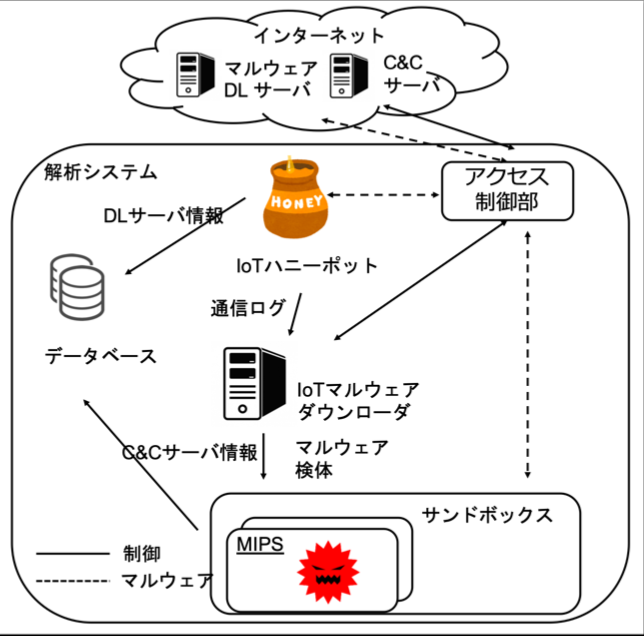
\includegraphics[width=6cm]{images/【調査】IoTボットネットのC2サーバに関して/experiment_environment.png}
    \caption{解析システムの構成図}
    \label{fig:experiment_environment}
\end{figure}

解析システムは5つの要素で構成されており, それぞれ以下の役割を持つ. 

\begin{description}
    \item[IoTハニーポット]~\\
    攻撃者によるログインの試みや侵入後のコマンドシーケンスを観測するために, 
    脆弱性のある10台のルータとWi-Fiストレージで構築されたハニーポット
    \item[IoTマルウェアダウンローダ]~\\
    IoTハニーポットで観測されたコマンドシーケンスからマルウェアをダウンロードするコマンドを抽出し, 
    攻撃者のダウンロードサーバからマルウェアの検体をダウンロードする
    \item[サンドボックス]~\\
    仮想環境とIoT機器の両方を用いて構成されており, サンドボックス上でマルウェアを実行する
    \item[アクセス制御部]~\\
    動的解析時の通信により攻撃に加担しないように, 
    IoTハニーポット, IoTマルウェアダウンローダ, サンドボックスとインターネット間の通信を制御する
    \item[データベース]~\\
    観測された攻撃者のサーバ情報やダウンロードしたマルウェアのバイナリ, その他関連する情報を保存する
\end{description}

\section{実験結果}
実験の結果, 6,295種類のマルウェアの検体を収集でき, 2,869件のC2サーバを観測することができた. 

\section{制御インフラに関して}
\subsection{C2サーバについて}
観測した多くのC2サーバを調べてみると, そのほとんどがクラウドサービス上のサーバを利用して運用していることが判明した. 
また, その生存期間は5日以内に7割, 2週間以内に9割近くのC2サーバが活動しなくなった. 

\subsection{マルウェアが持つC2サーバの情報について}
動的解析の結果, 1つのC2サーバに接続できない場合にべつのC2サーバに接続を試みるマルウェアが760検体存在した. 
これは攻撃者はマルウェア内にC2サーバのIPアドレスリストやドメインをハードコーディングされており, 
C2サーバに接続できなくなってもそれらを使って感染端末をコントロールすることができるようにしているからである. 
またC2サーバへの接続機能について静的解析を行ったところ, 1,443検体にはC2サーバに関する情報を1つしか持っておらず, 
C2サーバへの接続機能は脆弱であることがわかった. 

\section{考察}
実験の結果, IoT機器を標的とするマルウェアに関して, C2サーバとの接続に必要な情報を最小限にしか持っておらず, 
かつ短期間でC2サーバとの通信は行えなくなり, 攻撃者はボットネットを制御する手段を失うことがわかった. 
そのため, 攻撃者は攻撃を行う際に新たにC2サーバを用意し, IoT機器をマルウェアに感染させてボットネットを構築する, 
ということを繰り返していると考えられる. これは, IoT機器の多くでファームウェアの更新が十分でなく, 
容易にマルウェアに感染させることが可能であることが理由として挙げられる. また原らの研究\cite{原悟史2019感染持続型}から, 
IoTマルウェアの多くでは機器を再起動によって感染前の状態に戻すことができることから, 
攻撃者が感染状態の維持困難であることも理由のひとつだと考えられる. \par
このことから, IoTボットネットの大半は攻撃に利用されるとすぐに使い捨てられると考えられる. 

\section{おわりに}
玉井らの研究から, IoTボットネットのC2サーバの多くはクラウドサービスで運用されていることがわかった. 
また, 短い期間しか稼働しないにも関わらず, マルウェアのバイナリにはC2サーバへの接続情報が1つしか含まれていないことから, 
多くのIoTボットネットは使い捨てられてると考えられる. \par
今後は, IoT機器を対象としたボットネットのC2サーバのみではなく, Windowsなどのシステムも標的としたボットネットの
制御サーバに関する情報(検知回避手法, レスポンスステータスコードなど)について集めて, ボットネットとC2サーバの通信を
検知やその後の対策に利用したいと思う. 

\bibliographystyle{junsrt}
\bibliography{DB}
\end{document}